\documentclass[tikz,border=2mm]{standalone}
\usetikzlibrary{matrix,backgrounds}

\begin{document}
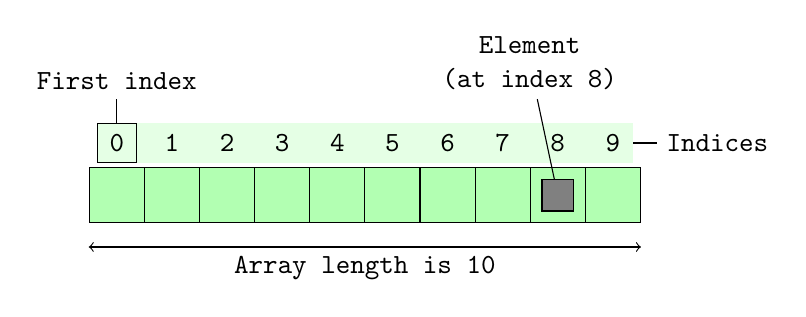
\begin{tikzpicture}[font=\ttfamily,
array/.style={matrix of nodes,nodes={draw, minimum size=7mm, fill=green!30},column sep=-\pgflinewidth, row sep=0.5mm, nodes in empty cells,
row 1/.style={nodes={draw=none, fill=none, minimum size=5mm}},
row 1 column 1/.style={nodes={draw}}}]

\matrix[array] (array) {
0 & 1 & 2 & 3 & 4 & 5 & 6 & 7 & 8 & 9\\
  &   &   &   &   &   &   &   &   &  \\};
\node[draw, fill=gray, minimum size=4mm] at (array-2-9) (box) {};

\begin{scope}[on background layer]
\fill[green!10] (array-1-1.north west) rectangle (array-1-10.south east);
\end{scope}

\draw[<->]([yshift=-3mm]array-2-1.south west) -- node[below] {Array length is 10} ([yshift=-3mm]array-2-10.south east);

\draw (array-1-1.north)--++(90:3mm) node [above] (first) {First index};
\draw (array-1-10.east)--++(0:3mm) node [right]{Indices};
\node [align=center, anchor=south] at (array-2-9.north west|-first.south) (8) {Element\\ (at index 8)};
\draw (8)--(box);
%
\end{tikzpicture}
\end{document}